\documentclass[a4paper, 12pt]{report}
\usepackage[T1]{fontenc}
\usepackage[utf8]{inputenc}
\usepackage[english]{babel}
\usepackage{mathtools}
\usepackage{amsfonts}
\usepackage{amsmath}
\usepackage{mathrsfs}
\usepackage{enumitem}
\usepackage{booktabs}
\usepackage{array}
% Avoid paragraph indent
\setlength{\parindent}{0pt}
% Useful floor and ceiling functions
\DeclarePairedDelimiter{\floor}{\lfloor}{\rfloor}
\DeclarePairedDelimiter{\ceil}{\lceil}{\rceil}
% Modified margins
\usepackage[margin=2cm]{geometry}
% This avoids hypenation
\hyphenpenalty=10000
\usepackage{tikz}
\usetikzlibrary{arrows,calc,positioning,shadows,shapes}
\usepackage{graphicx}
\usepackage{subfig}
\captionsetup[figure]{labelfont={bf},name={Figure},labelsep=period}
\captionsetup[table]{labelfont={bf},name={Table},labelsep=period}

\usepackage{float}


\begin{document}
	
\title{Digital Communications and Laboratory \\ Second Homework}
\author{Faccin Dario, Santi Giovanni}
\date{}
\maketitle

\section*{Problem 1}

\section*{Problem 2}

A flat fading channel with only one top $h_0(nT_c)$ was studied, assuming a \textit{Rice factor} of k=2 dB and normalized $M_{h_0}$. Moreover, a classical \textit{Doppler Spectrum} with $f_d T_c=40\cdot10^{-5}$ was considered. The schematic model to generate the coefficient $h_0$ of the channel is given in Figure \ref{Model_2}.

\begin{figure}[H]
	\centering
	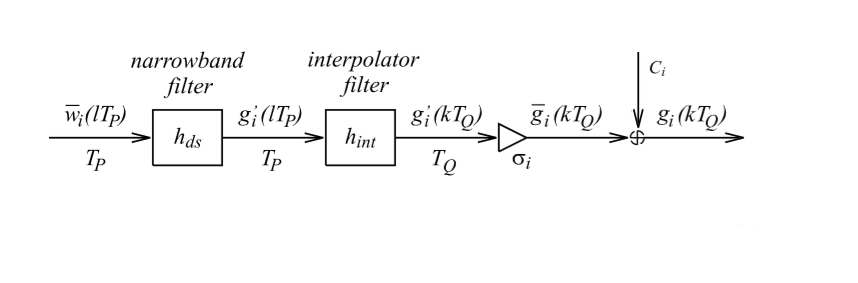
\includegraphics[width=14cm]{images/Model_2}
	\caption{Model to generate the coefficient $h_0$ of the time-varying channel.}\label{Model_2} 
\end{figure}

The Doppler Spectrum can be generated using a filter $h_{ds}$ such that $|\mathcal{H}_{ds}(f)|^2 = D(f)$.\\
In Table \ref{iircoeffs} are shown the coefficients used for such filter \cite{nevio<3}:

\begin{table}[H]
	\centering
	\begin{tabular}{c c c c}
		\toprule
		\textbf{$H_{ds}(z) = B(z)/A(z)$} & $f_dT_p=0.1$ &  &     \\
		\midrule
		$ \{a_n\} $ ,& $n=0, \dots, 11$:  & & \\
		1 & -4.4153 & 8.6283 & -9.4592   \\
	    6.1051 & -1.3542 & -3.3622 & 7.2390 \\
	    -7.9361 & 5.1221 & -1.8401 & 2.8706e-1 \\
	    \midrule
	    $ \{b_n\} $ ,& $n=0, \dots, 21$:  & & \\
	    1.3651e-4 & 8.1905e-4 & 2.0476e-3 & 2.7302e-3 \\
	    2.0476e-3 & 9.0939e-4 & 6.7852e-4 & 1.3550e-3 \\
	    1.8076e-3 & 1.3550e-3 & 5.3726e-4 & 6.1818e-5 \\
	    -7.1294e-5 & -9.5058e-5 & -7.1294e-5 & -2.5505e-5 \\
	    1.3321e-5 & 4.5186e-5 & 6.0248e-5 & 4.5186e-5 \\
	    1.8074e-5  & 3.0124e-6  & & \\
	    \bottomrule			
	\end{tabular}
	\caption{Coefficients for the IIR filter}
	\label{iircoeffs}
\end{table}


The graphical representation of the impulse response of the IIR filter and the Doppler Spectrum is shown in Fig. \ref{DS}. 
To obtain $h_0$, following the scheme of Fig. \ref{Model_2}, the noise component $w\sim \mathcal{CN}(0,1)$ is filtered with the IIR filter previously described. Note that the frequency response of this filter is $\mathcal{H}_{ds}(f)=\sqrt{\mathcal{D}(f)}$ while the PSD of the noise is constant and equal to 1. For this reason, the equivalent impulse response of this part is equal to $\mathcal{D}(f)=1\cdot |\mathcal{H}_{ds}|^2$ which is actually the Doppler spectrum. \\
The output of the filter is affected by a transient, which we avoided by considering only values after $5N_{eq}T_p$, where $N_{eq} = \left\lceil -\frac{1}{\ln(|p|)} \right\rceil$ is the equivalent time constant, and $p$ is the pole with the highest magnitude. Then, after scaling the coefficient such that $M_{h_0}/\sqrt{E_{h_{ds}}}=1$, the signal is filtered with an interpolation filter of factor $1/T_Q = T_p/T_c=250$. \\
The interpolator output signal is multiplied by a constant $\sigma_0 = \sqrt{M_d}$ to impose the desired power delay profile, and finally added up with another constant, $C$, which included the deterministic component according to \cite{nevio<3}, Page 307. The final signal is given in Fig. \ref{h0_7500}.

\begin{figure}[H]
	\centering
	\subfloat{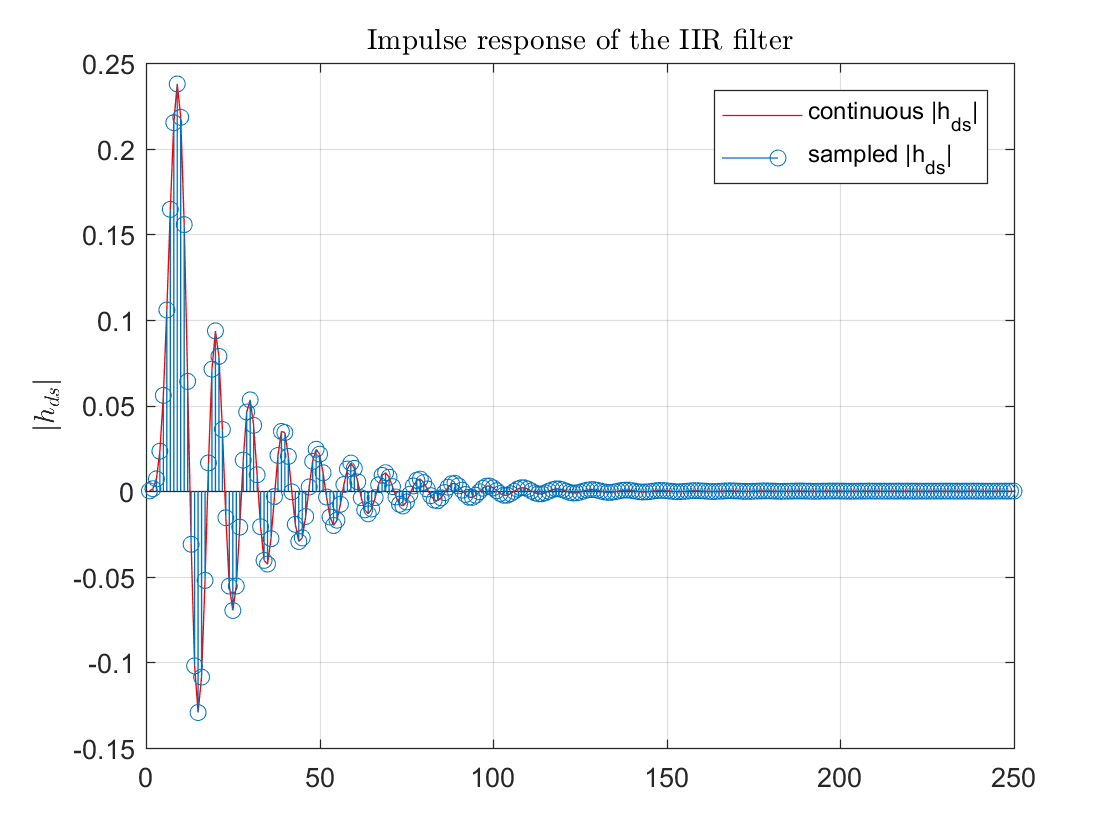
\includegraphics[width=7.5cm]{images/h_d}}
	\subfloat{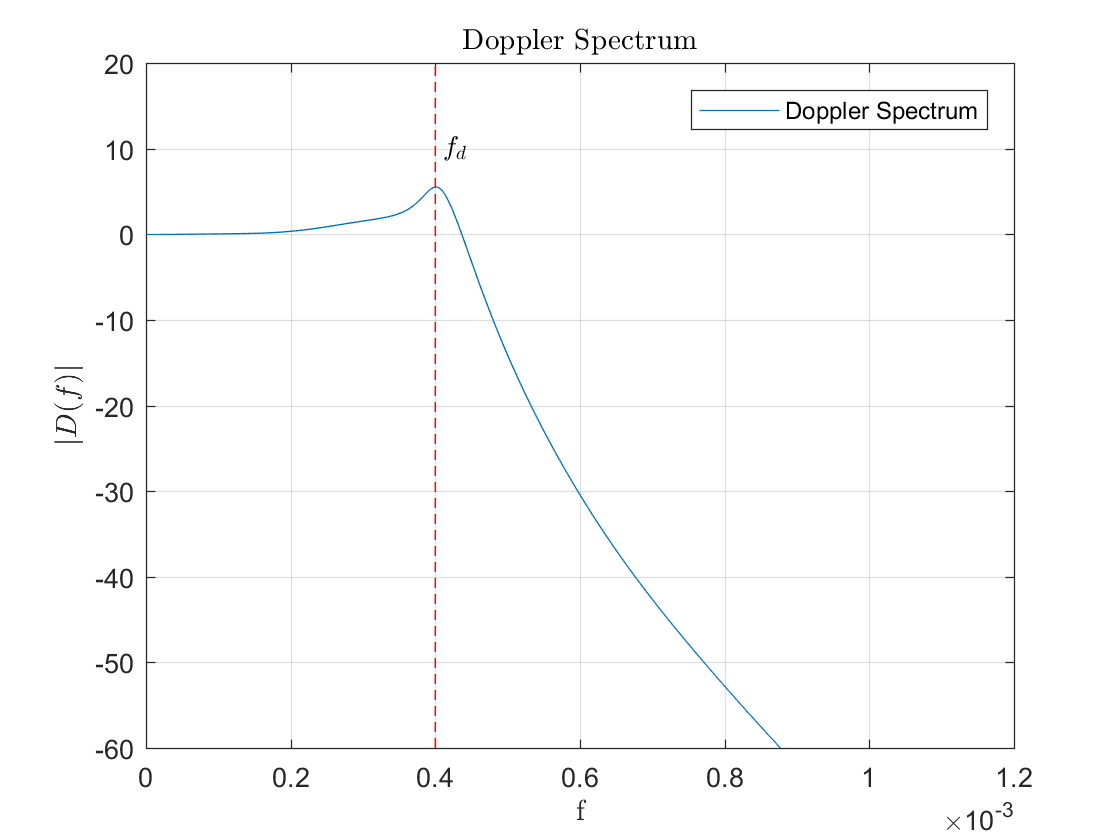
\includegraphics[width=7.5cm]{images/D}}
	\caption{Impulse response of the IIR filter and Doppler Spectrum}
	\label{DS}
\end{figure}

\begin{figure}[H]
	\centering
	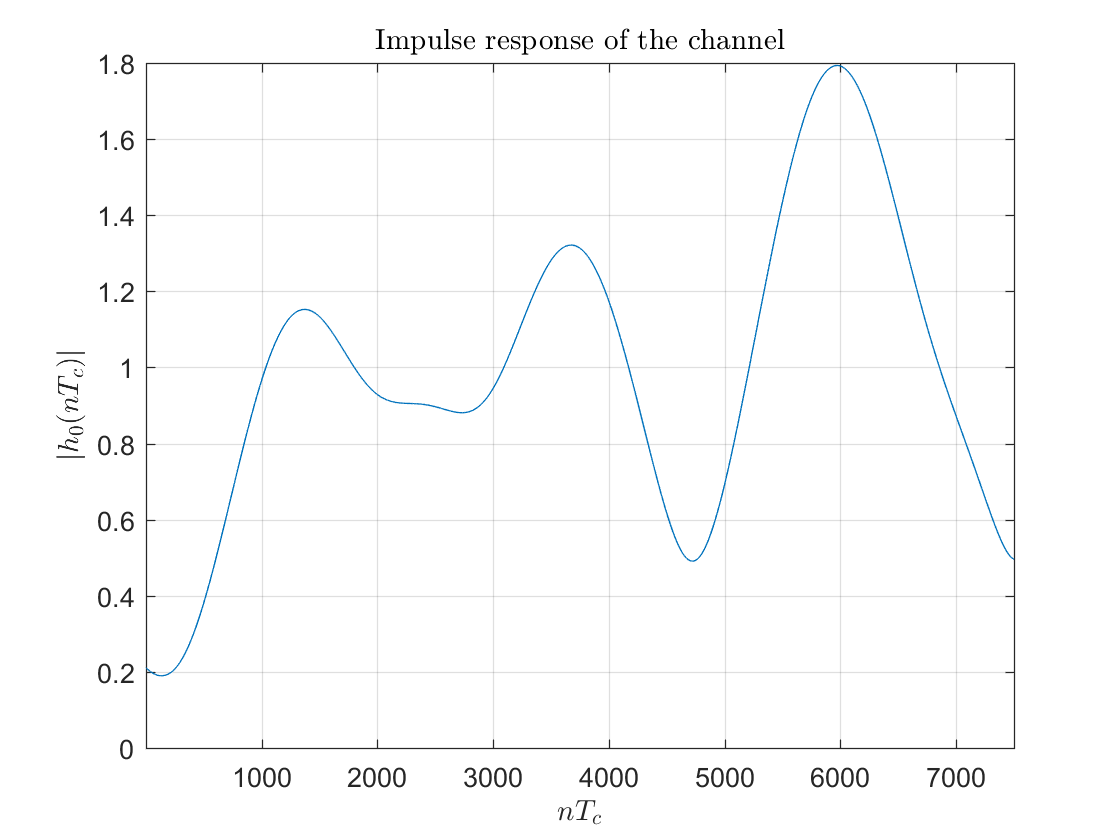
\includegraphics[width=14cm]{images/h0_7500}
	\caption{Magnitude of the simulated $h_0$ for 7500 samples.}\label{h0_7500}
\end{figure}

\clearpage
\subsection*{PDF of $\mathbf{\frac{|h_0|}{\sqrt{M_{|h_0|}}}}$}
The signal $h' = \frac{h_0}{\sqrt{M_{|h_0|}}} $ for 80000 samples is now studied. Note that, according to Fig. [\ref{Model_2}], $h'$ contains a deterministic component in addiction to a random component, which is complex gaussian with zero-mean and variance equal to one. For this reason the \textit{pdf} of $|h'|$ is a Rice distribution given by
\begin{equation}\label{Rice}
p_{|h'|} = \begin{cases*}
			2(1+K)ae^{-K-(1+K)a^2}I_0(2a\sqrt{K(1+K)}) \quad\quad a\ge0 \\
			0 \quad\quad\quad\quad\quad\quad\quad\quad\quad\quad\quad\quad\quad\quad\quad\quad\quad\quad\quad otherwise
\end{cases*}
\end{equation}

where $I_0$ is the \textit{modified Bessel function of the first type and order zero}, respectively
\begin{equation*}
I_0 = \frac{1}{2\pi}\int_{-\pi}^{pi}e^{x \cos \alpha}d\alpha
\end{equation*}

The histogram of $h'$ is shown in Figure [\ref{hist}]. Here it is given also the theoretical \textit{pdf} evaluated according to equation \ref{Rice}.

\begin{figure}[H]
	\centering
	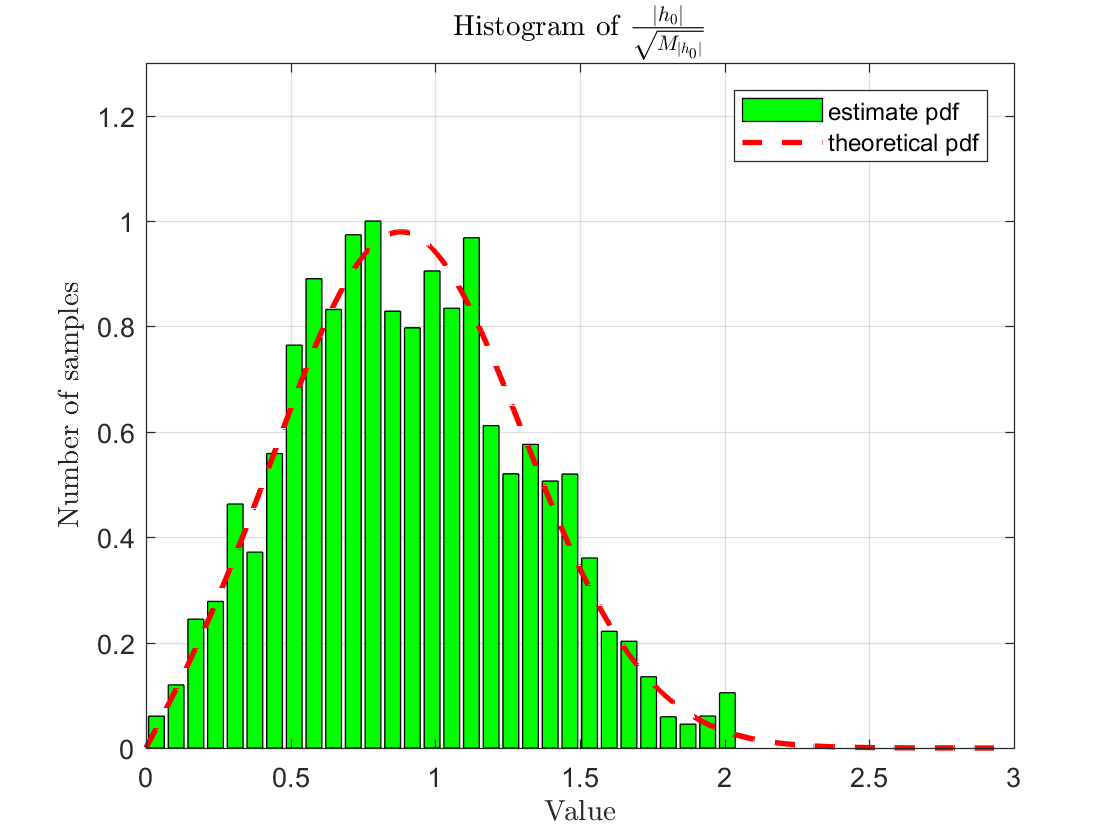
\includegraphics[width=14cm]{images/hist}
	\caption{Plot of both estimate and theoretical curve of the pdf of $h'$ .}\label{hist}
\end{figure}

\clearpage
\subsection*{Spectrum of $\mathbf{h_0}$}
In this section the spectrum oh $h_0$ is computed using the Welch Periodogram. This method extracts different subsequences of consecutive D samples which eventually overlap, and for each of these it computes the periodogram $\mathcal{P}_{PER}^{\left(s\right)}(f)$. The matematical model is given by
\begin{equation*}
\mathcal{P}_{WE}(F) = \frac{1}{N_s}\sum_{x=0}^{N_s-1}\mathcal{P}_{PER}^{(s)}(f)
\end{equation*}
where $N_s = \lfloor \frac{K-D}{D-S}-1 \rfloor$ is the total number of subsequences. \\
In order to compare the estimate with the theoretical case, the ideal PSD is computed. It is defined as the Fourier Transform of the autocorrelation function, which was evaluated using the unbiased estimator of equation \ref{autoc}:
\begin{equation}\label{autoc}
\hat{r}_x(n) = \frac{1}{K-n}\sum_{k=n}^Kh_0(k)h_0^*(k-n)  \quad\quad\quad n=0,1,\cdots,K-1
\end{equation}


\begin{thebibliography}{15}
	\bibitem{nevio<3}
	Nevio Benvenuto, Giovanni Cherubini,
	\textit{Algorithms for Communication Systems and their Applications}. 
	Wiley, 2002.
\end{thebibliography}

\end{document}